\documentclass{article}
\usepackage{listings}
\usepackage{xcolor}

\title{GAE}
\author{Do Viet Anh BI12-024}

\maketitle

\begin{document}

\lstset{language=Python,
        basicstyle=\ttfamily\footnotesize,
        breaklines=true,
        keywordstyle=\color{blue},
        stringstyle=\color{red},
        commentstyle=\color{green},
        showstringspaces=false,
        numbers=left,
        numberstyle=\tiny,
        frame=single,
        captionpos=b}

\section{Important snippets}
\begin{enumerate}
    \item \textbf{Initialization of the Sudoku board:} The \texttt{\_\_init\_\_} method initializes the Sudoku board with a $9 \times 9$ grid filled with zeros.
   
    \item \textbf{Printing the board:} The \texttt{print\_board} method prints the current state of the Sudoku board in a visually appealing format with appropriate row and column separators.
    
    \item \textbf{Validity checks for moves:} Methods like \texttt{is\_valid\_row}, \texttt{is\_valid\_col}, and \texttt{is\_valid\_subgrid} check whether a move is valid based on Sudoku rules.
    
    \item \textbf{Main game loop:} The \texttt{main} function sets up the game, generates a full Sudoku board, removes a certain number of cells to create the puzzle, and then enters a loop where the player can input their moves until the puzzle is solved.
\end{enumerate}

\section{How structure code}
\begin{enumerate}
    \item \textbf{Class Definition:} The code defines a \texttt{Sudoku} class, encapsulating all functionalities related to the Sudoku game.
    
    \item \textbf{Methods for Generating and Solving Sudoku:} The \texttt{generate}, \texttt{solve}, and \texttt{generate\_full\_board} methods are placeholders for functionalities related to generating and solving Sudoku puzzles. Currently, they are empty and need to be implemented.
    
    \item \textbf{Input and Output Handling:} The \texttt{print\_board} method handles the visual representation of the Sudoku board, while the \texttt{main} function takes user input for row, column, and number, checks the validity of the move, updates the board accordingly, and prints the updated board.
    
    \item \textbf{Game Loop:} The main game loop in the \texttt{main} function keeps the game running until the puzzle is solved. Within this loop, the user is prompted to input their moves, and the board is updated accordingly.
    
    \item \textbf{Conditional Check for Puzzle Completion:} The code checks if there are no zeros left on the board to determine if the puzzle has been solved, indicating that all cells have been filled correctly.
\end{enumerate}

\section{Results}

Here are the results:

\begin{figure}[h]
  \centering
  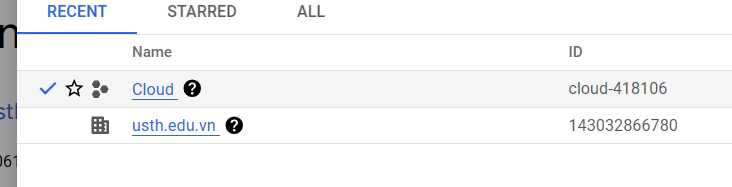
\includegraphics[width=0.8\textwidth]{create_prj.png}
  \caption{Create project and set up python environment}
\end{figure}

\begin{figure}[h]
  \centering
  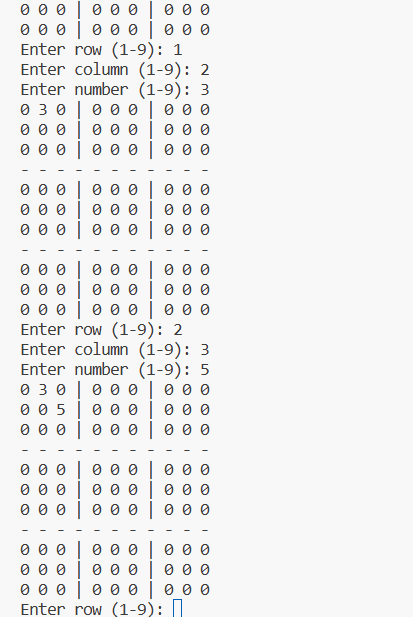
\includegraphics[width=0.8\textwidth]{result.png}
  \caption{Result of soduky.py}
\end{figure}

\end{document}

